\section{Model programowy transformaty Hougha}

\blindtext

\subsection{Model funkcjonalny z użyciem OpenCV}

Do budowy wysokopoziomowego modelu funkcjonalnego użyte zostały funkcje biblioteki OpenCV:\\*
\texttt{void Canny(InputArray image, OutputArray edges, double threshold1, double threshold2, int apertureSize=3)} \\*

gdzie \\*
\texttt{image} – obraz wejściowy \\*
\texttt{edges} – wyjściowy obraz do detekcji krawędzi, \\*
\texttt{threshold1} – pierwszy próg binaryzacji,\\*
\texttt{threshold2} – drugi próg binaryzacji,\\*
\texttt{apertureSize} – rozmiar maski użytej w funkcji \texttt{Sobel()}.\\*

\texttt{void HoughLines(InputArray image, OutputArray lines, double rho, double theta, int threshold, double srn=0, double stn=0 )} \\*
\texttt{image} – binarny obraz wejściowy, \\*
\texttt{lines} – wyjściowy wektor linii; każda reprezentowana jest przez dwa elementy – $\rho$ i $\theta$ \\*
\texttt{rho} – krok dla odległości $\rho$ w pikselach \\*
\texttt{theta} – krok dla kąta $\theta$ w radianach \\*
\texttt{threshold} – próg głosów, które musi osiągnąć linia aby została zwrócona. \\*

% 3 obrazki obok siebie
\begin{figure}[!htb]
\minipage{0.32\textwidth}
  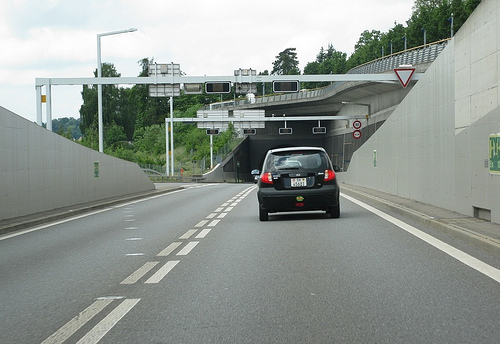
\includegraphics[width=\linewidth]{img/road4.jpg}
  \caption{Obraz z kamery}\label{fig:awesome_image1}
\endminipage\hfill
\minipage{0.32\textwidth}
  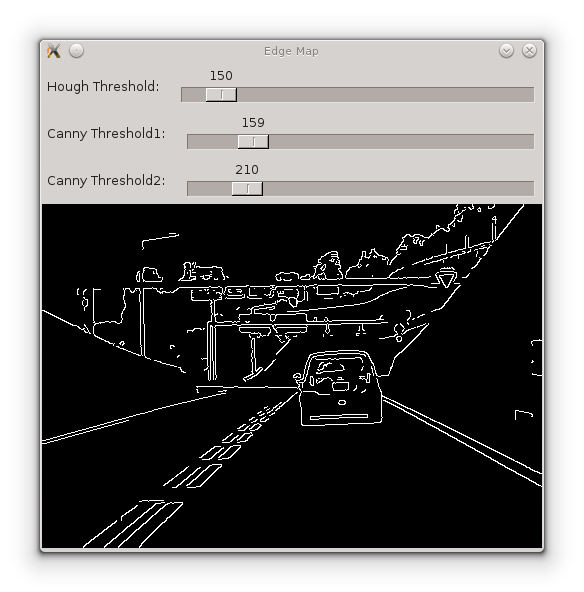
\includegraphics[width=\linewidth]{img/canny_screen.png}
  \caption{Krawędzie znalezione metodą Canny}\label{fig:awesome_image2}
\endminipage\hfill
\minipage{0.32\textwidth}%
  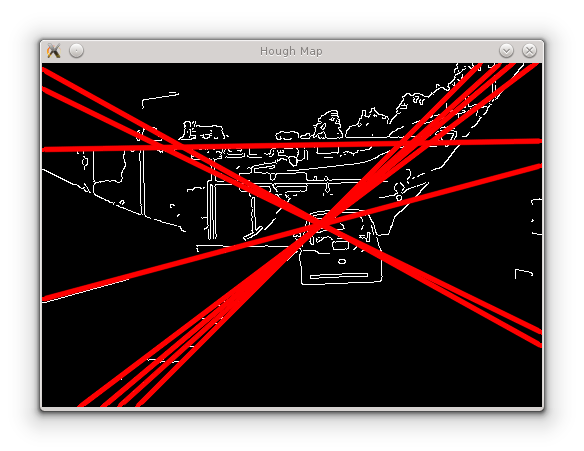
\includegraphics[width=\linewidth]{img/hough_screen.png}
  \caption{Linie wybrane przez transformatę Hougha z głosowaniem}\label{fig:awesome_image3}
\endminipage
\end{figure}

\blindtext

%
%\begin{figure}[!htb]
%\centering
%\includegraphics[scale=1]{img/start2.png}
%\caption{Rozwiązanie przed optymalizacją z wektorem przełączeń $\tau = [0.015, 0.035, 0.055]$}
%\label{rys:start1}
%\end{figure}

\newpage
\subsection{Model stałoprzecinkowy w języku C++}

Opis programu

Klasa \texttt{fp.h}

\begin{figure}[!htb]
\centering
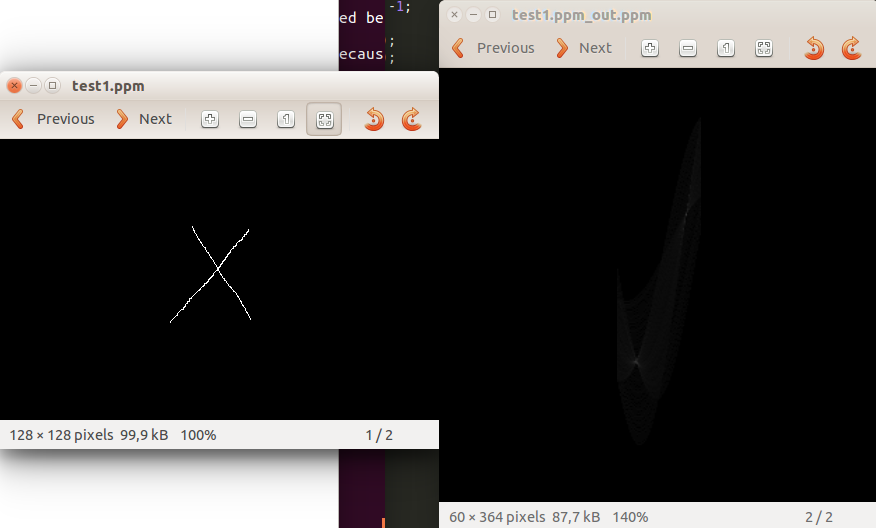
\includegraphics[scale=0.75]{img/fixed.png}
\caption{Wynik działania funkcji \texttt{Hough()} dla liczb stałoprzecinkowych}
\label{rys:fp}
\end{figure}

